
\begin{table*}[t]
\centering
\begin{tiny}
\begin{tabular}{|l|l|l|l|l|l|l|}
\hline
{\bf Dataset}	& {\bf Size} & {\bf Prediction} & {\bf \#Features} & {\bf \#Protected} & {\bf Protected Feature Types} & {\bf Baseline}\\ \hline
Communities and Crime  & 1994 & High Violent Crime ? & 128 & 18 & Race & 0.3 \\ \hline
Law School	       & 2053 & Pass Bar Exam ? & 10 & 4 & Race, Income, Age, Gender & 0.49 \\ \hline
Student		       & 396  & Course Performance ? & 30 & 5 & Age, Gender, Relationship, Alcohol Use & 0.47 \\ \hline
Adult		       & 2021 & Income $>=$ \$50K ? & 14 & 3 & Age, Race, Gender & 0.50 \\ \hline
\end{tabular}
\end{tiny}
\caption{Description of Data Sets.}
\label{tab:datasets}
\end{table*}

\section{Empirical Evaluation}


In this section, we describe an extensive empirical investigation of the $\knrw$ algorithm on
four datasets in which fairness is a potential concern.
Among the questions of primary interest are the following:
\begin{itemize}
\item Does the $\knrw$ algorithm work in practice, despite the use of imperfect heuristics for the Learner and Auditor?
\item Is the notion of subgroup fairness interesting empirically, in that there are palatable trade-offs between accuracy
	and subgroup fairness (as opposed to it
	being too strong a constraint, and thus resulting in a very steep error increase for even weak subgroup fairness)?
\end{itemize}
We will answer these questions strongly in the affirmative, which is perhaps the overarching message of our results.
We also carefully compare subgroup fairness to standard marginal fairness, and show that optimizing
	for the latter in general does poorly on the former --- thus something like the $\knrw$ algorithm is actually necessary
	to achieve subgroup fairness.

More generally, aside from performance, we provide a number of empirical analyses that elucidate
	the underlying behavior and convergence properties of the $\knrw$ algorithm, and discuss its strengths and
	weaknesses.

\subsection{Datasets}

We ran experiments on $3$ datasets from the UCI Machine Learning
Repository \cite{UCI}:
\textbf{Communities and Crime} \citep{communities},
\textbf{Adult},
and \textbf{Student} \citep{student}, and the \textbf{Law School} dataset from the Law School Admission Council's National Longitudinal Bar Passage Study \citep{lawschool}.
These datasets were selected due to their potential fairness concerns, including:
\begin{itemize}
\item Data points representing individual people (or in the case of Communities and Crimes,
	small U.S. communities of people);
\item The presence of features capturing properties often associated with possible
	discrimination, including race, gender, and age;
\item Potential sensitivity of the predictions being made, such as violent crime,
	income, or performance in school.
\end{itemize}

The properties of these datasets are summarized in Table~\ref{tab:datasets},
including the number of instances, the prediction being made, the overall number of
features (which varies from 10 to 128),
the number of protected features in the subgroup class (which varies from 3 to 18),
the nature of the protected
features, and the baseline (majority class) error rate.

Some methodological notes:
\begin{itemize}
\item We note that two of the datasets (Law School and Adult) were initially much larger
but were extremely imbalanced with respect to the predicted label, making sensible
error comparisons numerically difficult. We thus randomly downsampled these two datasets to
obtain approximately balanced prediction problems on each.
\item All categorical variables have been preprocessed with a one-hot encoding.\item The $\knrw$ algorithm has two input parameters: the maximum allowed subgroup fairness violation.
	$\gamma$, and a tuning parameter $C$ which represents (in the theoretical derivation in \cite{KNRW18}) an upper bound on the magnitude of the dual variables needed to express the fairness constrained empirical risk minimization problem.
	We view $\gamma$ as an important control variable allowing us to explore the tradeoff between
	fairness and accuracy, and thus will vary it in our experiments. On the other hand, $C$ is more of a
	nuisance parameter, and thus for consistency and simplicity we set $C = 10$ in all experiments.
	Experimentation with larger values of $C$ did not reveal qualitatively different findings on the
	datasets investigated.
\item We emphasize that {\em all results are reported in-sample on the datasets\/}, and thus we are treating
	the empirical distributions of the datasets as the ``true'' distributions of interest. We do this
	because our primary interest is simply in examining the performance and behavior of the $\knrw$ algorithm
	on the actual data or distributions, and not in generalization per se. As noted in~\cite{KNRW18},
	theoretical generalization bounds for both error and subgroup fairness
	can be obtained by standard methods, and will depend on (e.g.) the
	VC dimension of the Learner's model class $\cH$ and the Auditor's subgroup class $\cF$. As usual,
	we would expect empirical generalization to often be considerably better than the worst-case theory.
\end{itemize}

\subsection{Empirical Convergence of $\knrw$}
\label{subsec:conv}

\begin{center}
\begin{figure*}[h]
\centering
\subfigure[]{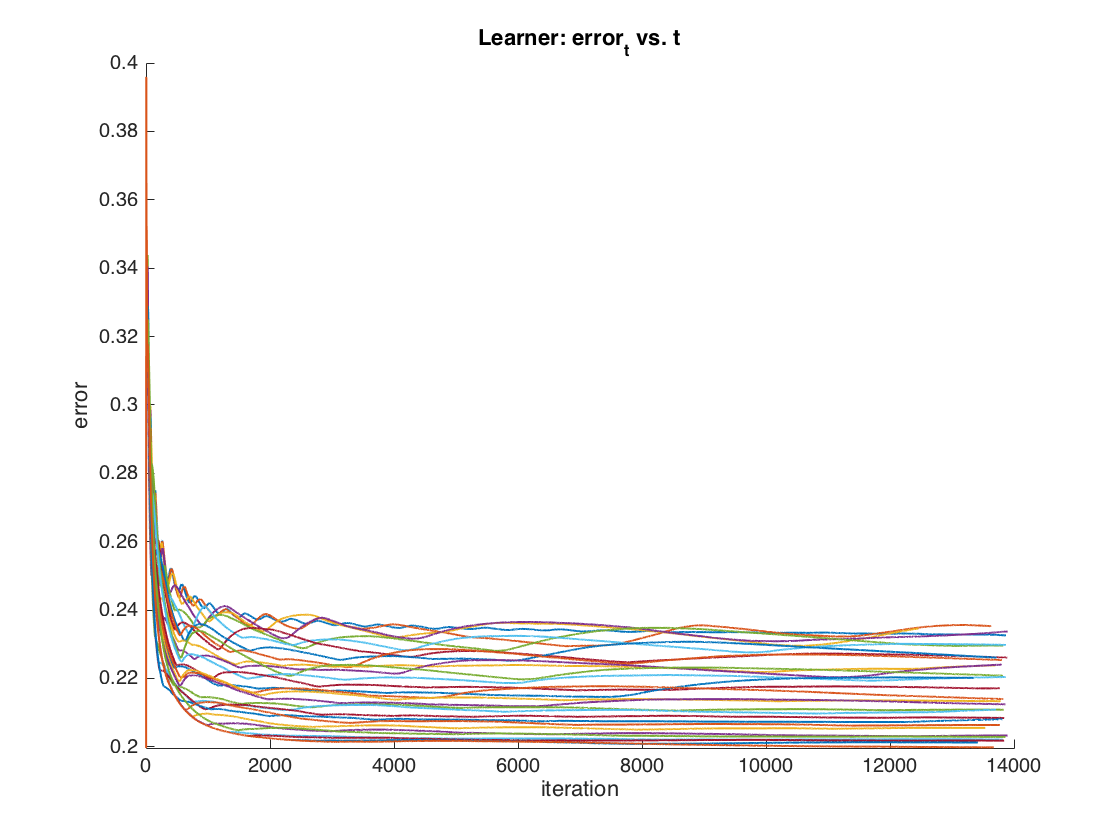
\includegraphics[scale=0.2]{figures/lawerraug8.png}}
\subfigure[]{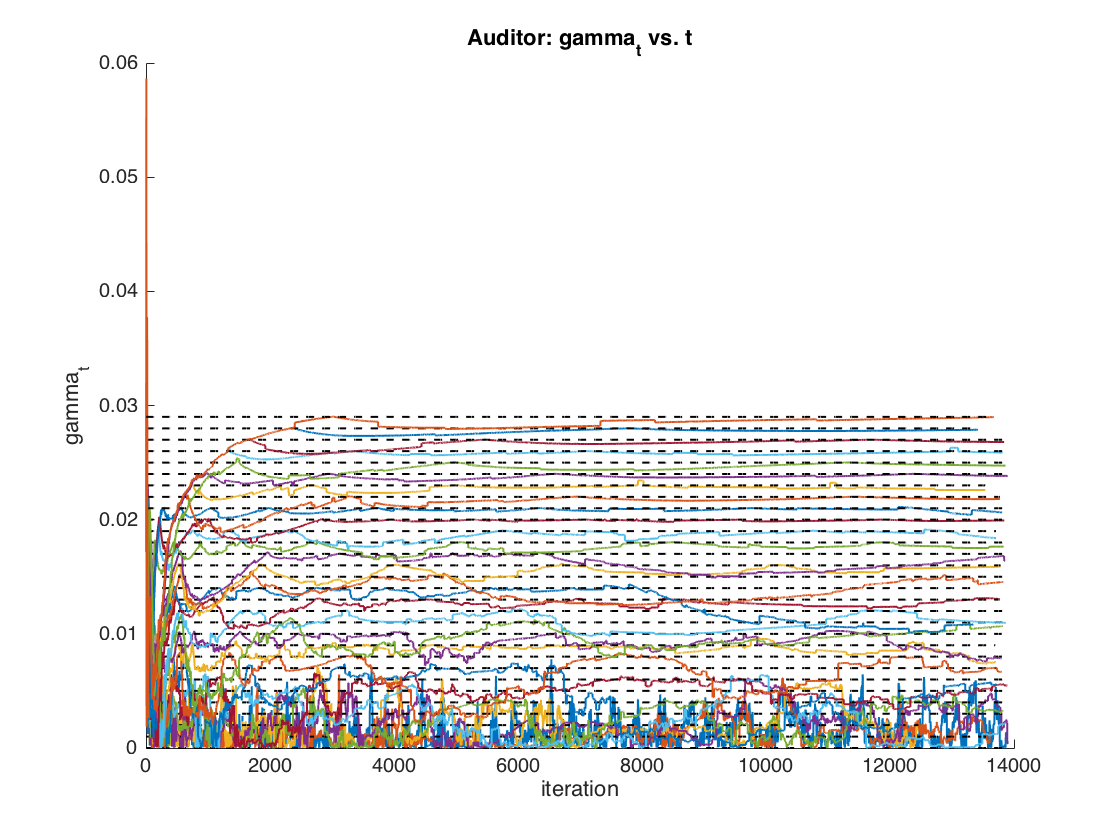
\includegraphics[scale=0.2]{figures/lawgamaug8.png}}
\subfigure[]{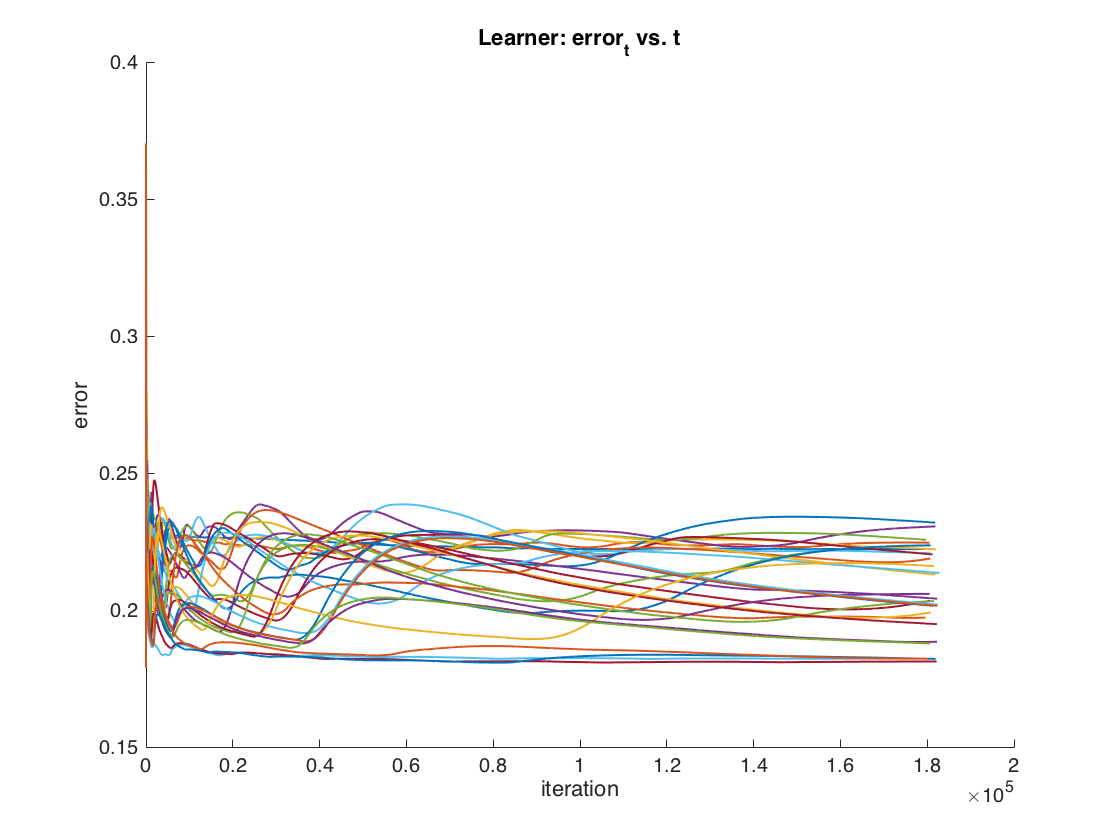
\includegraphics[scale=0.2]{figures/adulterraug8.png}}
\subfigure[]{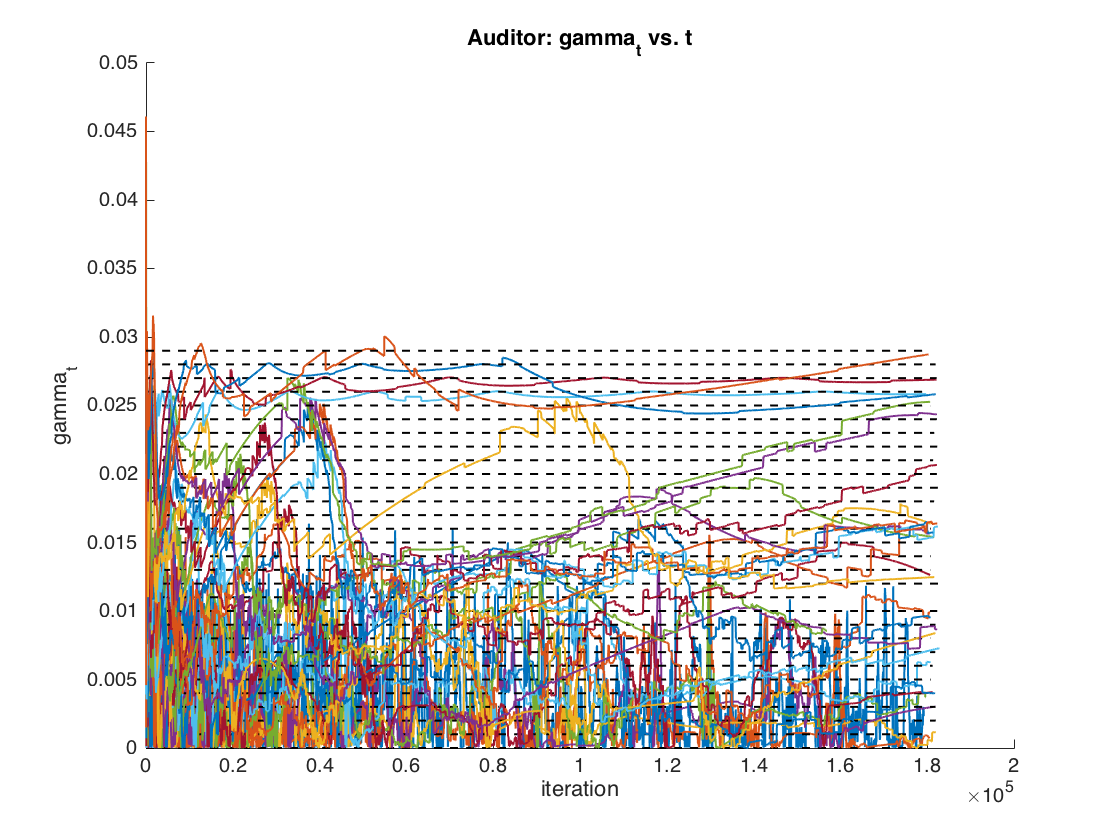
\includegraphics[scale=0.2]{figures/adultgamaug8.png}}
\caption{{Error $\epsilon_t$ and fairness violation $\gamma_t$ for Law School dataset (panels (a) and (b)) and Adult data set
(panels (c) and (d)), for values of input $\gamma$ ranging from 0 to 0.03.
Dashed horizontal lines on $\gamma_t$ plots correspond to varying values of $\gamma$.
}}
\label{fig:conv}
\end{figure*}
\end{center}

We begin with an examination of the convergence properties of the $\knrw$ algorithm on the four datasets.
\citet{KNRW18} had already reported preliminary convergence results for the Communities and Crime dataset,
showing that their algorithm converges quickly, and that varying the input $\gamma$ provides an appealing trade-off between
error and fairness.
In addition to replicating those findings for Communities and Crime,
we also find that they are not an optimistic anomaly.
For example, for the Law School dataset, in Figure~\ref{fig:conv} %\footnote{
%For most of the figures in our investigation,
%we are mainly interested in qualitative properties, so in the interests of
%space we have made the images small.
%Numerical detail can be viewed by zooming in, and is also discussed in the
%text when relevant.
%}
we plot both the error $\epsilon_t$ (panel (a)) and the fairness violation
$\gamma_t$ (panel (b)) as a function of the iteration $t$, for values of the input $\gamma$ ranging from 0 to 0.03.
We see that the algorithm converges relatively quickly (on the
order of thousands of iterations), and that
increasing the input $\gamma$ generally yields decreasing error and increasing fairness violation (typically saturating
the input $\gamma$), as suggested
by the idealized theory.

But on other datasets the empirical convergence does not match the idealized theory as cleanly, presumably due to the
use of imperfect Learner and Auditor heuristics. In panels (c) and (d) of Figure~\ref{fig:conv} we again plot $\epsilon_t$
and $\gamma_t$, but now for the Adult dataset. Even after approximately 180,000 iterations, the algorithm does not appear
to have converged, with $\epsilon_t$ still showing long-term oscillatory behavior, $\gamma_t$ exhibiting extremely noisy
dynamics (especially at smaller input $\gamma$ values), and there being no clear systematic, monotonic relationship between
the input $\gamma$ and error acheived. But despite this departure from the theory, it remains the case that varying $\gamma$
still yields a diverse set of $\langle \epsilon_t, \gamma_t \rangle$ pairs, as we will see in the next section.
In this sense, even in the absence of convergence
the algorithm can be viewed as a valuable search tool for models trading off accuracy and fairness.

Overall, we found rather similar convergent behavior on the Communities and Crime and Law School datasets, and
less convergent behavior on the Adult and Student datasets.


\iffalse
We now examine the convergence of the $\knrw$ Algorithm. We focus our discussion on two datasets that illustrate different modes of convergence: Communities \& Crime and Adult. In Figure~\ref{fig:conv} plots (a) and (c) show the iteration-by-iteration error of the Learner's classifier for Communities and Adult respectively, across a range of input $\gamma$ values from $0$ to $.026$, and $0$ to $.045$. Note the maximum $\gamma$ values correspond to the unfairness of the unconstrained classifier. Figures (b) and (d) show the evolution of the $\gamma$-unfairness over time, e.g. the $\gamma$-unfairness of the group found by the Auditor at each iteration. We now distinguish between the two cases.  \sn{why isn't there a horizontal line in (d) at the largest input gamma}

In Communities \& Crime error and $\gamma$ curves generally level out quickly -- by iteration $8000$ or so. The dashed lines in the $\gamma$ plots correspond to the input levels of $\gamma$, and since after initially being driven down towards $0$ the $\gamma$ values are converging to their input values, this indicates that the fairness constraint is saturated at convergence. As we would expect the final error achieved is monotonic with respect to the input values of $\gamma$; a lower $\gamma$ corresponds to a more stringent fairness constraint and hence a larger error. The base rate in Communities \& Crime is .3, and so we see over input $\gamma$ as small as $.001$ we achieve non-trivial error. Its difficult to visualize the exact trajectory of the $\gamma$ values prior to converging, and so we explore the joint convergence of error and $\gamma$ in the trajectory plots below.

In Adult the story is less clean. While error and $\gamma$ are driven down initially after the first few audits, we see more violations of monotonicity by input $\gamma$ through $20000$ iterations. For example, even though the purple line in (c) corresponds to an input $\gamma$ of $.024$ which is higher than the input gamma of $.023$ corresponding to the yellow line, we see that the yellow line has error lower than the purple line at iteration 20000. The $\gamma$ plots are also substantially noisier in the early iterations in plot (d), and we see many violations of input $\gamma$ even at iteration 20000. These differences are both indicative of a lack of convergence -- either by virtue of the oracles failing, the input value of $C$ being too low, or perhaps the Fictitious Play dynamic failing to converge. Nevertheless the silver lining is that even though the algorithm is clearly far from convergence, each model at each iteration for each input $\gamma$ still corresponds to an achievable (error, $\gamma$) pair. By taking the un-dominated Pareto frontier of (error, $\gamma$) pairs the algorithm still traces out a useful error-fairness tradeoff as we will see in Subsection~\ref{subsec:pareto}.
\fi

\subsection{Subgroup Pareto Frontiers and Comparison to Marginal Fairness}
\label{subsec:Pareto}

\begin{figure*}[p]
\centering
\subfigure[]{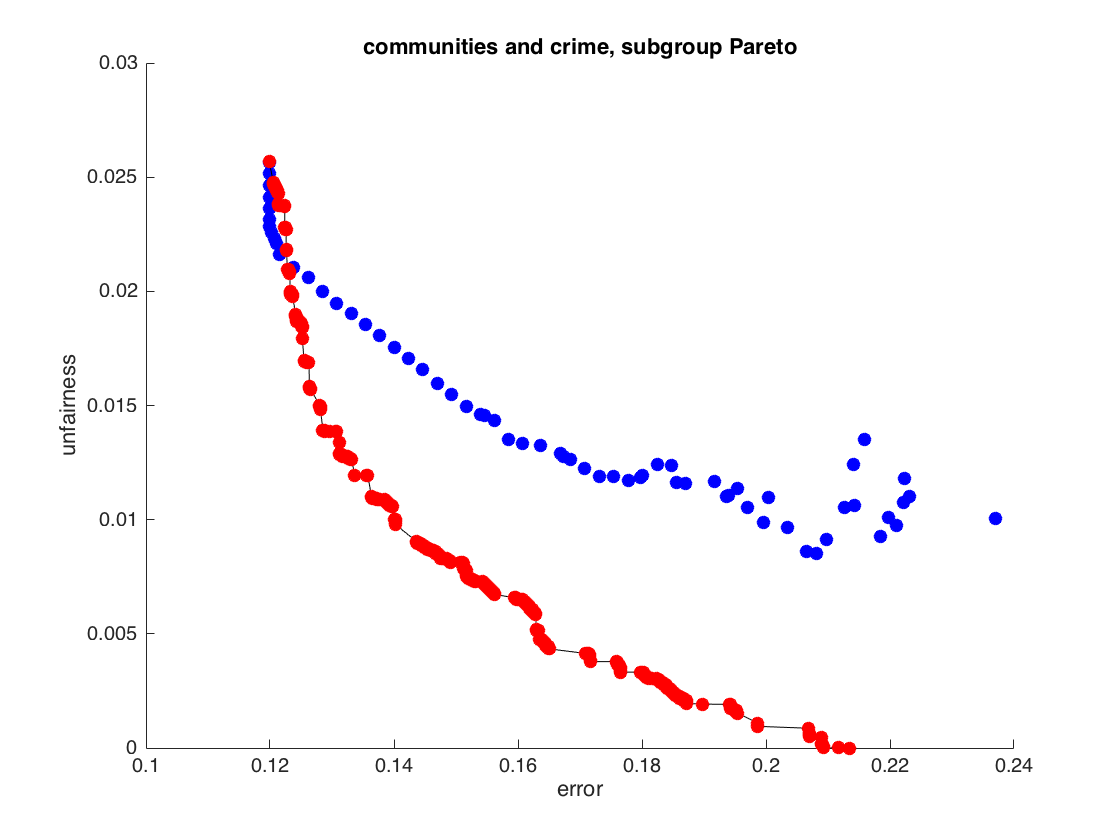
\includegraphics[scale=0.14]{figures/ccsubaug9.png}}
\subfigure[]{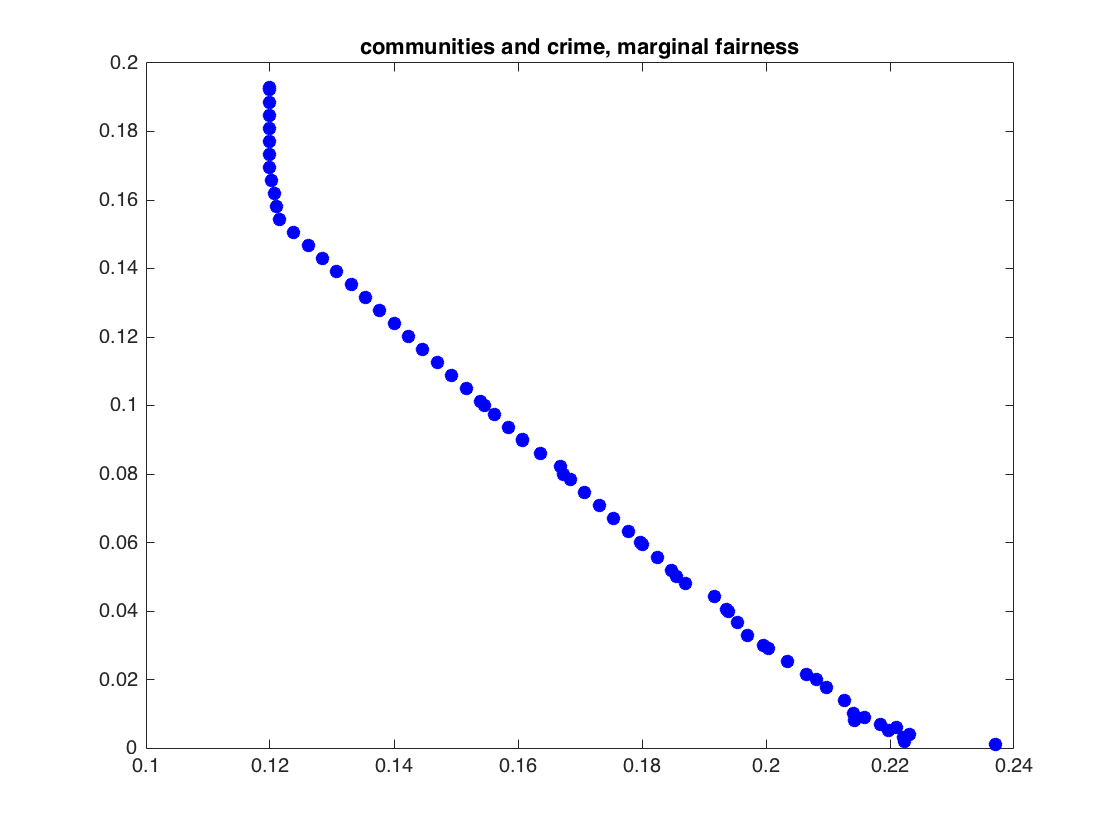
\includegraphics[scale=0.14]{figures/ccmaraug9.png}}
\subfigure[]{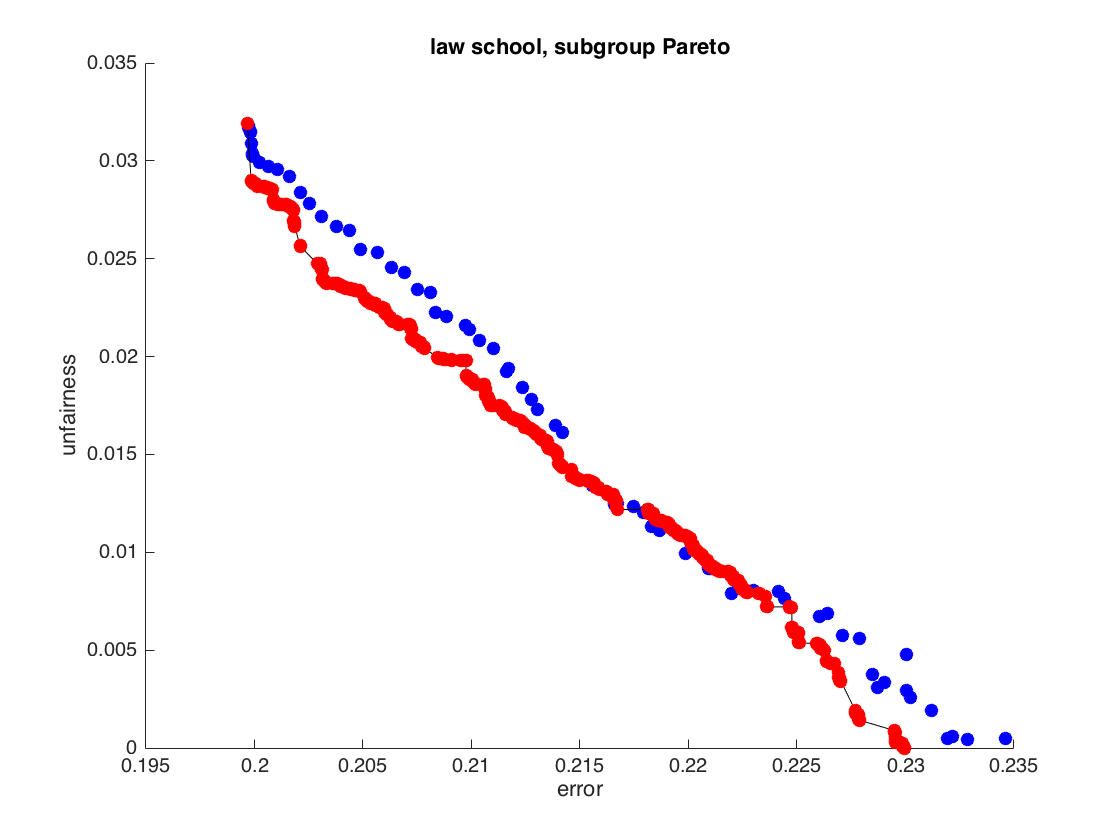
\includegraphics[scale=0.14]{figures/lawsubaug9.png}}
\subfigure[]{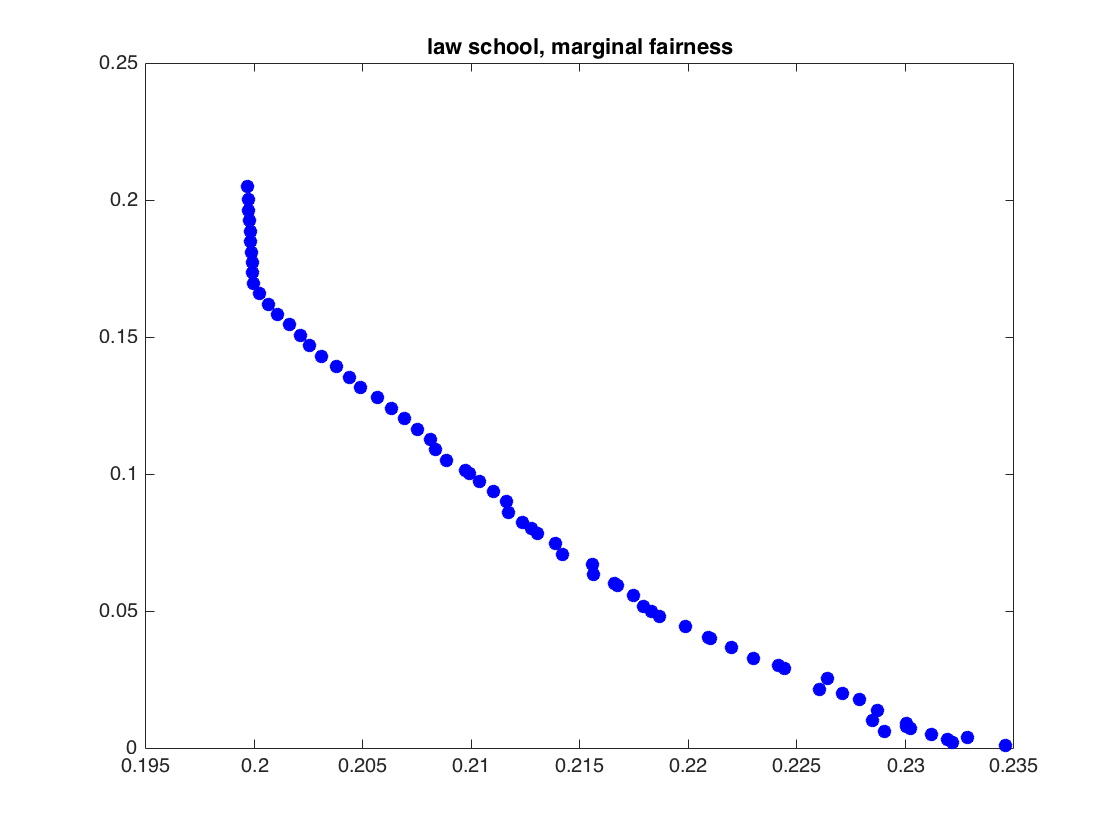
\includegraphics[scale=0.14]{figures/lawmaraug9.png}}
\subfigure[]{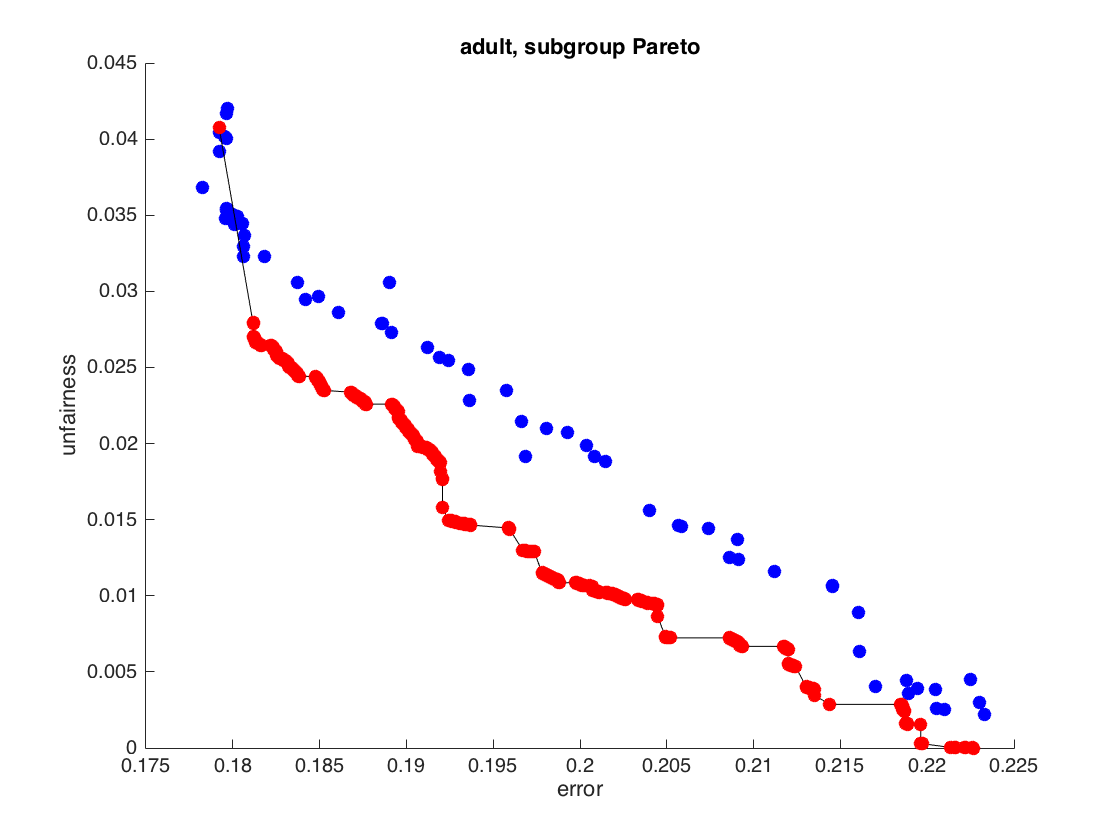
\includegraphics[scale=0.14]{figures/adultsubaug9.png}}
\subfigure[]{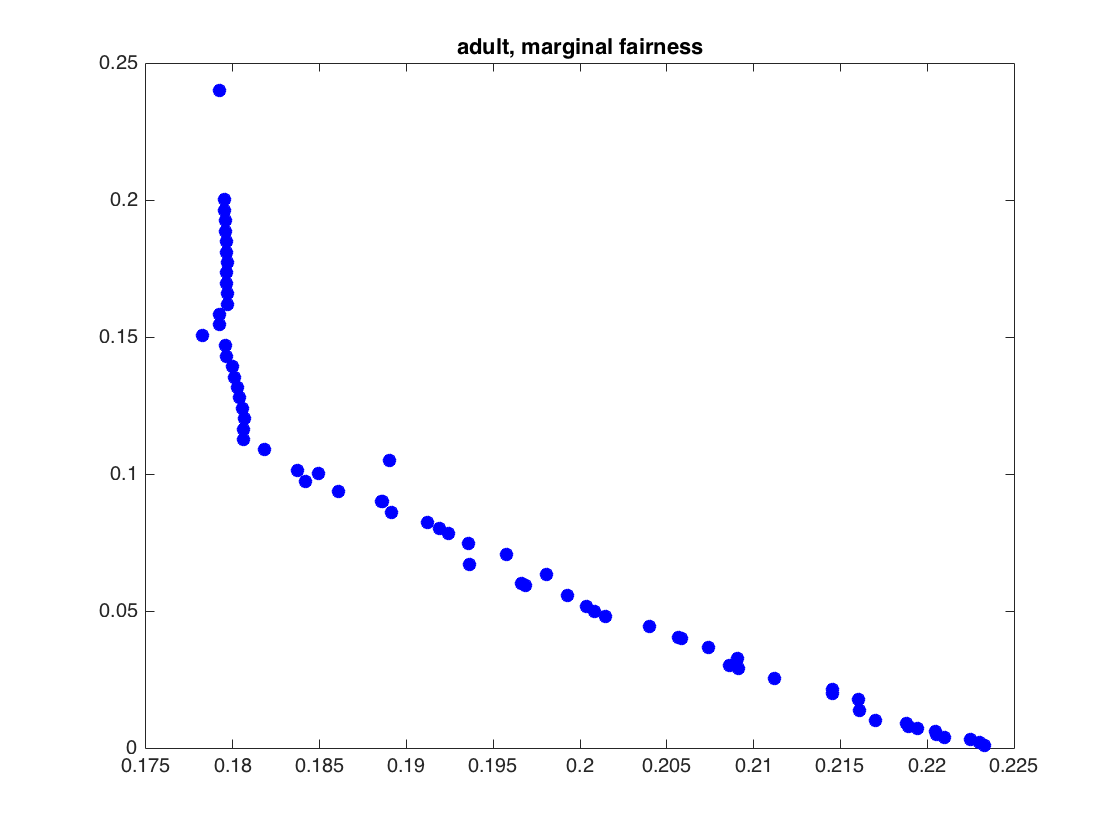
\includegraphics[scale=0.14]{figures/adultmaraug9.png}}
\subfigure[]{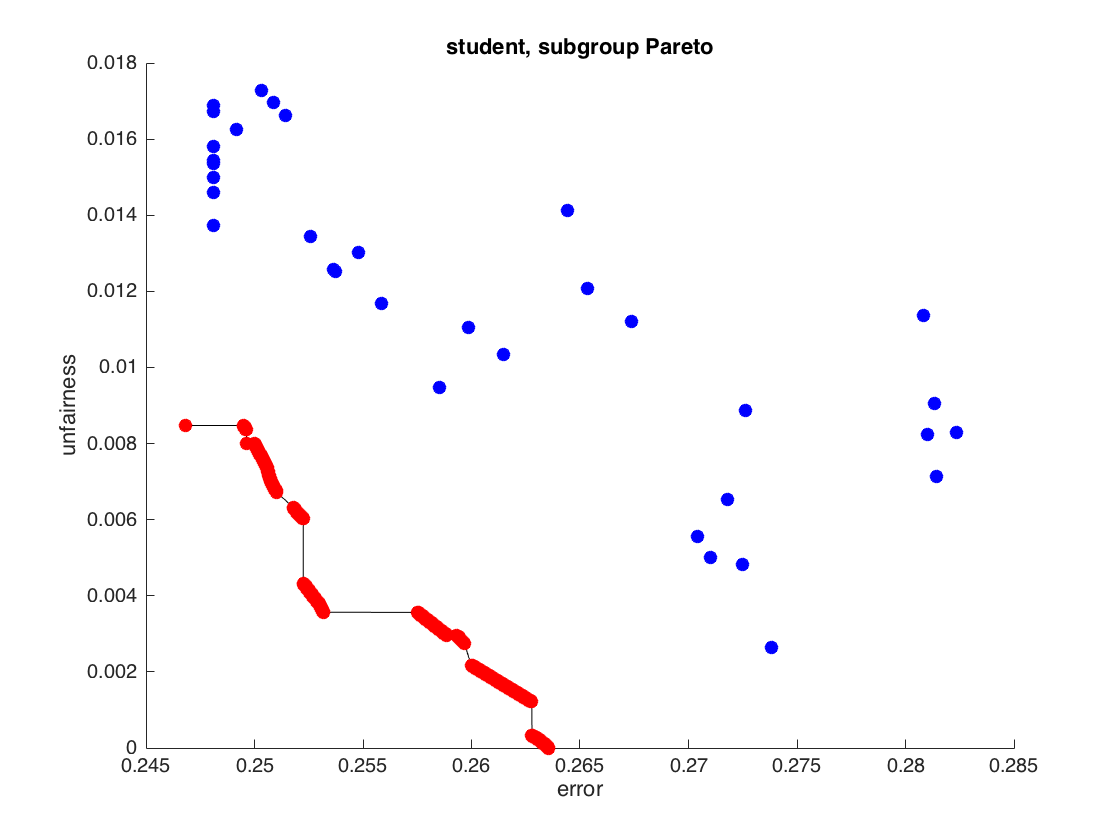
\includegraphics[scale=0.14]{figures/studentsubaug9.png}}
\subfigure[]{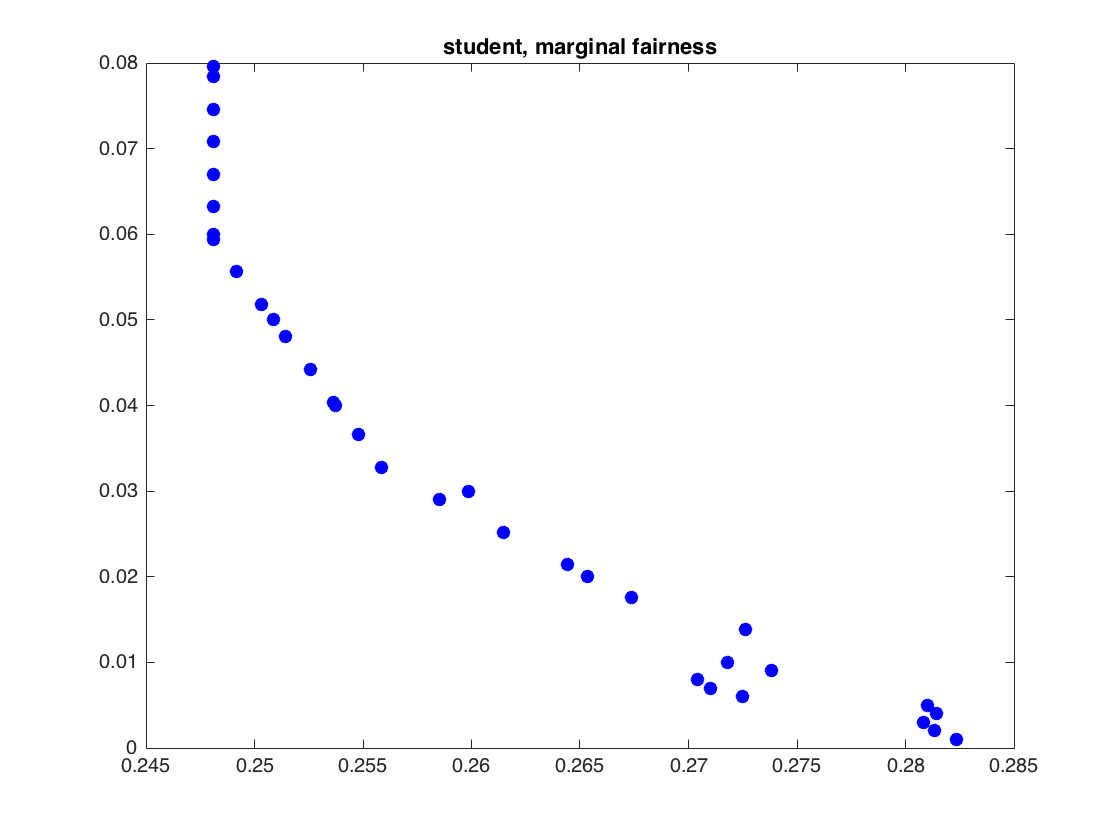
\includegraphics[scale=0.14]{figures/studentmaraug9.png}}
\caption{{Left column: The red points show the Pareto frontier of error (x axis) and subgroup fairness violation (y axis)
	for the $\knrw$ algorithm across all four data sets, while the blue points show the error and subgroup fairness violation
	for the models achieved by the $\MSR$ algorithm.
	Right column: The error and marginal fairness violation for the $\MSR$ algorithm across all four data sets.
	Ordering of datasets is Communities and Crime, Law School, Adult, and Student.}}
\label{ccpar}
\end{figure*}

Regardless of convergence, for plots such as those in Figure~\ref{fig:conv}, it is natural to take the
$\langle \epsilon_t, \gamma_t \rangle$
pairs across all $t$ and all input $\gamma$, and compute the undominated or Pareto frontier of these pairs.
This frontier represents the accuracy-fairness tradeoff achieved by the $\knrw$ algorithm on a given data set, which
is arguably its most important output. The choice of where one wants to be on the frontier is a policy question that should be made by
domain experts and stakeholders, and dependent on the stakes involved (e.g. online advertising vs. criminal sentencing).

It is also of interest to compare the subgroup fairness achieved by
the $\knrw$ algorithm (which is explicitly optimizing under a subgroup fairness constraint)
with an algorithm only optimizing under weaker and more
traditional marginal fairness constraints. To this end, we also implemented a version of the algorithm from \cite{MSR} --- which we will refer to as the $\MSR$ algorithm ---
for marginal
fairness.\footnote{Since some of the protected attributes are continuous rather than discrete, and the $\MSR$ algorithm only
handles discrete attributes, in order to run the marginal fairness algorithm we
create sensitive groups by thresholding on the mean of each sensitive attribute.}
% For example, given a sensitive attribute such as \textit{pctpolwhite} we construct two groups $g_{pctpolwhite}^{+}$ and its complement $g_{pctpolwhite}^{-}$, where a point is in $g_{pctpolwhite}^{+}$ if its value of the sensitive attribute  \textit{pctpolwhite} is greater than the mean of  \textit{pctpolwhite} in the population. This is how we run the $\MSR$ algorithm on all numeric sensitive attributes across all datasets.
From a theoretical perspective, {\em a priori\/}
we would expect models trained for marginal fairness to fare poorly on subgroup fairness. But it
is an empirical question --- perhaps on some datasets, demanding marginal fairness
already suffices to enforce subgroup fairness as well. Thus the high-level
question is whether the $\knrw$ framework and algorithm are worth the added analytical and computational overhead.

In the left column of Figure~\ref{ccpar}, we show the $\knrw$ algorithm Pareto frontiers for subgroup fairness on all four datasets, and also the pairs
achieved by the $\MSR$ algorithm. In the right column, we also separately show the
marginal fairness frontier achieved by the $\MSR$ algorithm. Before discussing the particulars of each dataset,
we first make the following general observations:
\begin{itemize}
\item For most datasets, the $\knrw$ algorithm yields a Pareto curve that frequently lies well below the straight line
	connecting its endpoints (which we can think of as an empirical form of strong convexity),
	and thus there are non-trivial tradeoffs between accuracy and fairness to consider. On some of these
	curves there are regions of steep descent where subgroup unfairness can be reduced significantly
	with negligible increase in error.
\item While the $\MSR$ algorithm performs well with respect to marginal fairness (right column) as expected, it fares much
	worse than the $\knrw$ algorithm on subgroup fairness for three of the datasets. Thus marginal fairness
	is not just theoretically, but also empirically a weaker notion, and generally will not imply subgroup fairness
	``for free''.
\item Nevertheless, there are a handful of points in which the $\MSR$ algorithm produces
	models that actually lie below (and thus dominate) the $\knrw$ Pareto curve by a small amount.
	While this is not possible under the idealized theory --- subgroup fairness is a strictly stronger
	notion than marginal fairness --- it can again be explained by the use of imperfect learning heuristics
	by both algorithms.
\item Focusing just on the $\MSR$ marginal fairness curves in the right column, we see that each of them
	begins with a steep drop, meaning that in every case, the marginal unfairness of the unconstrained
	error-optimal model can be significantly improved with little or no increase in error.
\item By matching points between the $\MSR$ marginal and subgroup fairness plots, we find that
	with the exception of the Student data set, there is a systematic relationship between marginal and
	subgroup unfairness: asking the $\MSR$ algorithm to reduce marginal unfairness also causes it to
	reduce subgroup unfairness --- but not by as much as the $\knrw$ algorithm achieves.
\end{itemize}
Together these observations let us conclude that subgroup fairness is a strong but achievable notion in practice
(at least on these datasets), and that the $\knrw$ algorithm appears to be an effective tool for its investigation.

It is also worth commenting on the differences across datasets, and focusing not just on the qualitative shapes of the
Pareto curves but their actual numerical specifics --- especially since in real applications, these will matter to stakeholders.
For instance, the actual range of error values spanned by the $\knrw$ Pareto curves ranges from nearly 10\% (Communities and Crime)
to less than 2\% (Student). So perhaps for Communities and Crime, the tradeoff is starker from an accuracy perspective. We now provide
some brief commentary on each dataset.\\

\noindent
{\bf Communities and Crime (panels (a) and (b)):}
This is the dataset with perhaps the cleanest and most convex $\knrw$ Pareto curve, with steep drops in subgroup unfairness possible
	for minimal error increase at the beginning.
	In particular are able to reduce the initial $\gamma$-unfairness
	from $0.026$ to less than $0.005$ while only increasing the error from $0.12$ to $0.16$.
	This is a meaningful reduction in unfairness -- e.g. reducing a $26\%$ percent difference
	in false positive rate on a subgroup comprising $10\%$ of the population,
	to a less than $5\%$ false positive rate disparity on a subgroup of the same size.
	Eventually the Pareto curve flattens out, resulting in increasing accuracy costs for reduced unfairness.
	While the $\MSR$ subgroup unfairness curve matches the $\knrw$ Pareto curve on the far left (for all datasets),
	since this corresponds to minimizing error unconstrained by any fairness notion, the outperformance by $\knrw$
	grows rapidly as we make stronger fairness demands.\\

\noindent
{\bf Law School (panels (c) and (d)):}
Here the $\knrw$ Pareto curve appears to be approximately linear, thus providing a constant tradeoff between accuracy and subgroup fairness.
	Interestingly, this is the one dataset in which asking for marginal fairness appears to also yield subgroup fairness for free,
	as the $\MSR$ curve lies very close to the $\knrw$ curve.
	Since this dataset has the fewest number of features overall and the second
	fewest number of protected features, one might be tempted to conjecture that when the
	number of protected features is small, guaranteeing marginal fairness approximately
	guarantees rich subgroup fairness. This claim is falsified by the fact that
	 on the Adult dataset which has similar dimensionality (see below), there is 
	a large gap between the $\knrw$ and $\MSR$ subgroup fairness curves.\\

\noindent
{\bf Adult (panels (e) and (f)):}
Here we see a less smooth $\knrw$ curve, possibly corresponding to the poorer convergence properties on this dataset mentioned earlier. Nevertheless,
	the numerical tradeoff exhibits regions of both steep, inexpensive reduction in unfairness and flat, costly reduction.
	$\MSR$ is again considerably worse when evaluated on subgroup fairness, but still shows a systematic relationship to marginal fairness.\\

\noindent
{\bf Student (panels (g) and (h)):}
Similar to Adult, a varied $\knrw$ curve with multiple tradeoff regimes. This is also the lone dataset in which reducing marginal
	fairness appears to have no relationship to subgroup fairness --- while the $\MSR$ marginal pareto curve in panel (h) remains
	relatively smooth, the subgroup fairness of the corresponding models in panel (d) is now not only worse than for $\knrw$,
	but shows no monotonicity.
	$\knrw$ is able to decrease $\gamma$-unfairness to $0$ with only a $2\%$ increase in error,
	while the $\MSR$ algorithm only drives the subgroup unfairness to $0.002$ at its best,
	with an over $3\%$ increase in error from the unconstrained classifier.\\

\iffalse
\begin{remark}
The attentive reader might wonder about the $\MSR$ models whose error is far to the right of models
	acheiving (estimated) subgroup fairness equal to zero, which happens on the law and student datasets. It turns out that
	these high-error $\MSR$ models have even *marginal* unfairness that is non-zero, suggesting that it is actually
	impossible we are acheiving zero subgroup unfairness at the same error, since marginal unfairness always lower bounds
	subgroup unfairness. The most likely explanation for this discrepancy is once again the heurstic nature of our auditor ---
	the models we measure as having zero unfairness probably do have some numerically small unfairness that is missed by
	the auditor. Nevertheless, again one would obviously prefer $\knrw$ to $\MSR$ as a search tool for models with low
	subgroup unfairness.
\end{remark}
\fi

\iffalse
Now lets quickly recap the themes that have emerged from the results on our four datasets:
\begin{itemize}
\item If strong subgroup fairness is the primary concern, $\knrw$ always outperforms $\MSR$ often significantly
\item Reducing marginal unfairness typically carries the added benefit of a monotonic decrease in strong subgroup fairness, though this is not guaranteed
\item The $\knrw$ algorithm was able to drive strong subgroup fairness to zero on all datasets and achieve non-trivial error, with the perfectly fair classifier having error between $2-10\%$ higher than the unconstrained classifier.
\item All marginal fairness fairness curves have a steep, nearly vertical initial decline; meaning it is possible to reduce their marginal unfairness by several $\%$ points with essentially no cost to accuracy.
\item While all Pareto curves are convex, the error-$\gamma$ tradeoff varies significantly from dataset to dataset
\end{itemize}
\fi

Having established the efficacy of subgroup fairness and the $\knrw$ algorithm on the four datasets,
we now turn to experiments and visualizations allowing us to better understand the behavior and dynamics
of the algorithm.

\subsection{Flattening the Discrimination Surface}
\label{subsec:heatmap}

%\begin{center}
\begin{figure*}[p]
\subfigure[]{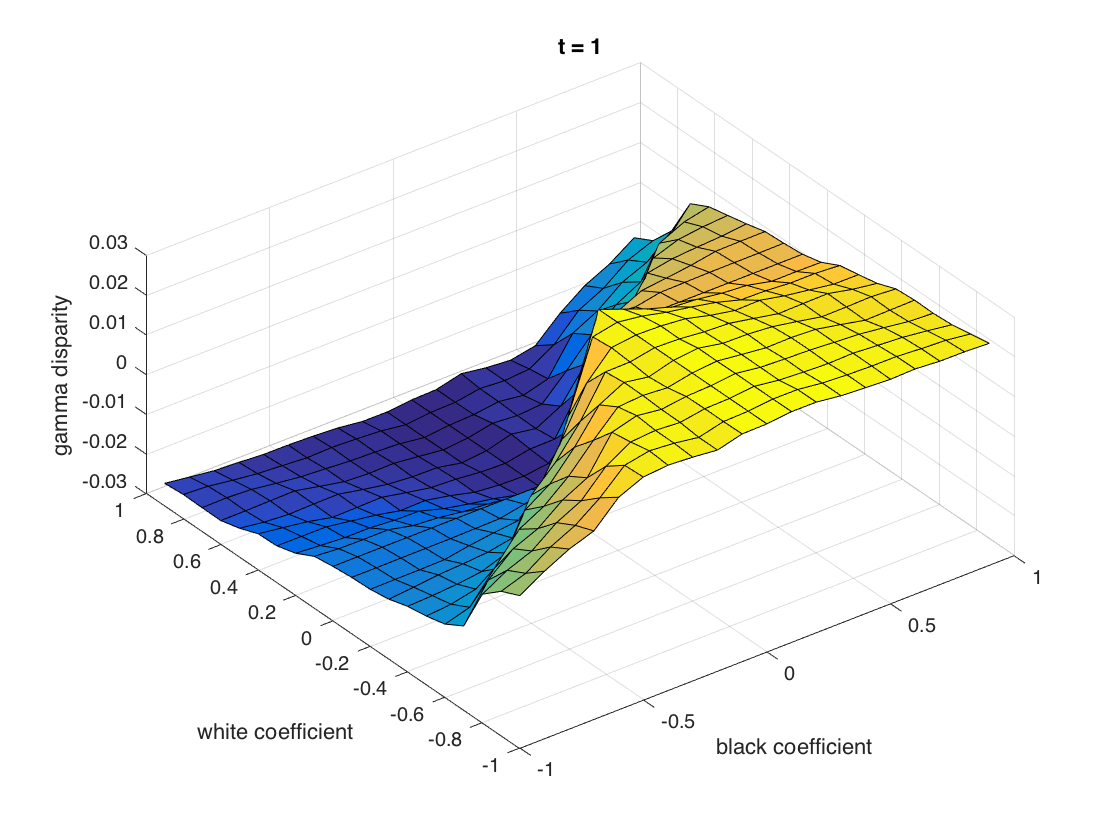
\includegraphics[scale=0.15]{figures/heatfig1.png}}
\subfigure[]{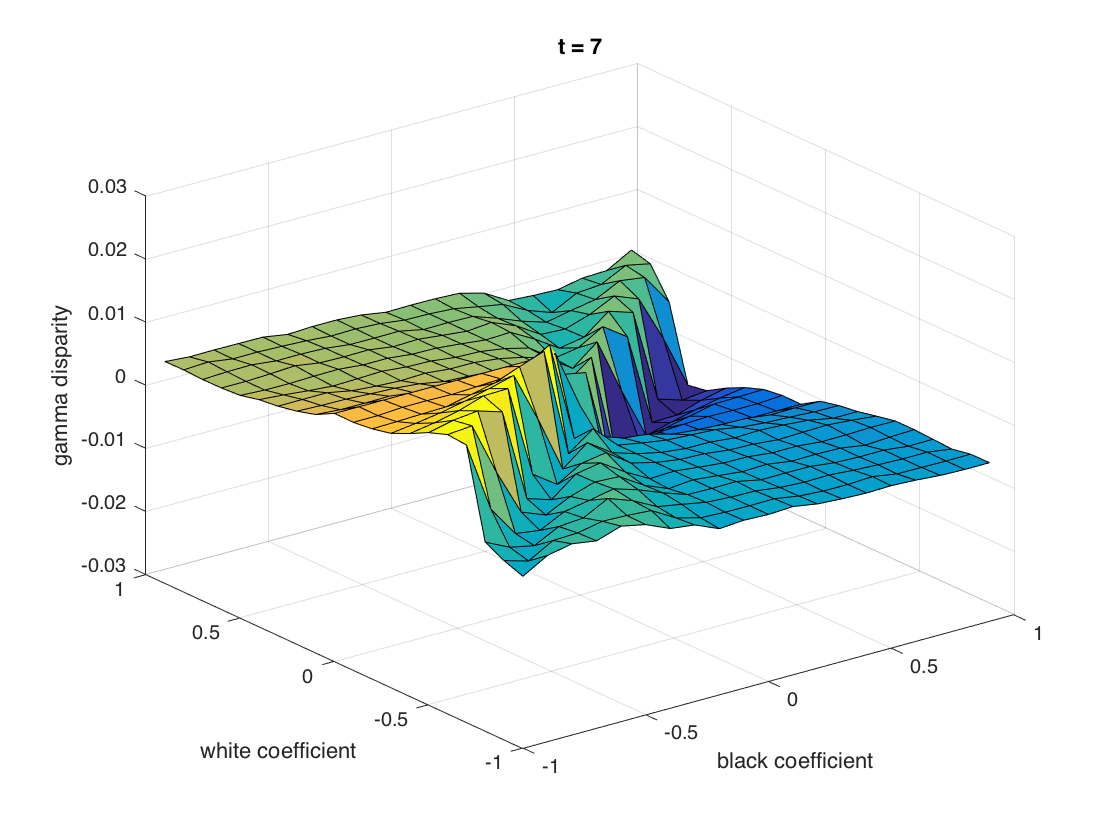
\includegraphics[scale=0.15]{figures/heatfig7.png}}
\subfigure[]{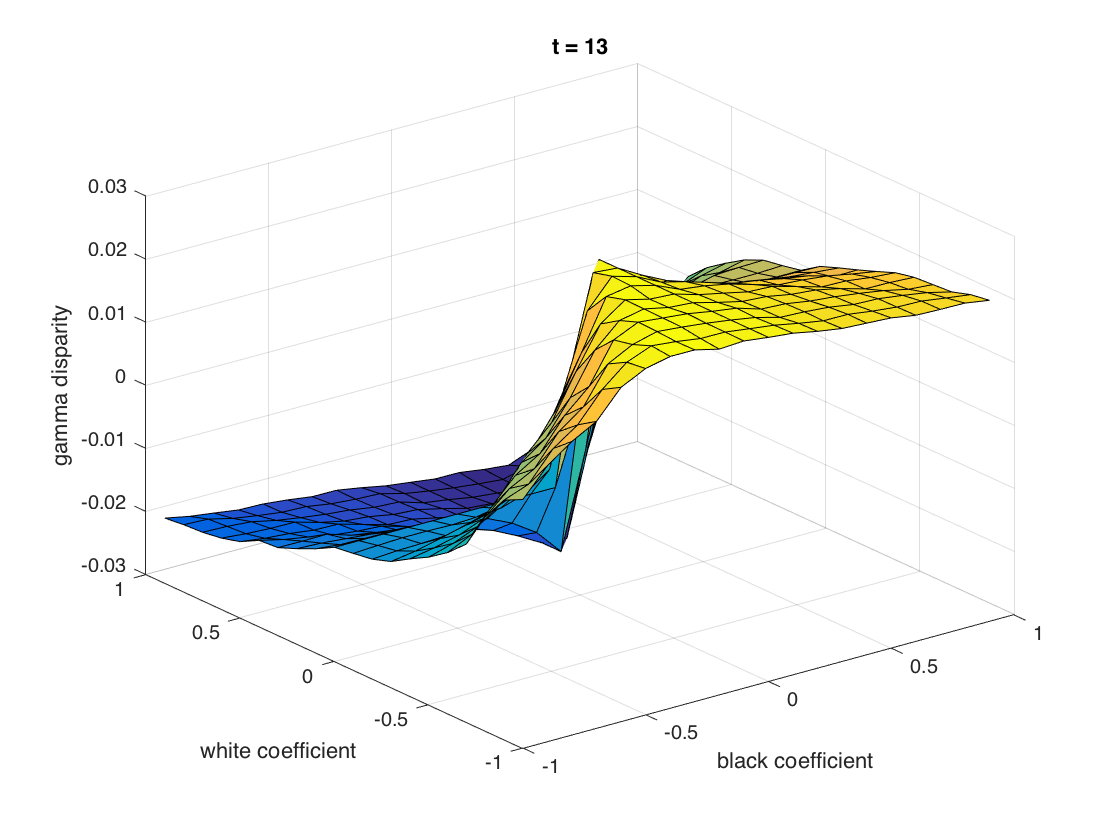
\includegraphics[scale=0.15]{figures/heatfig13.png}}
\subfigure[]{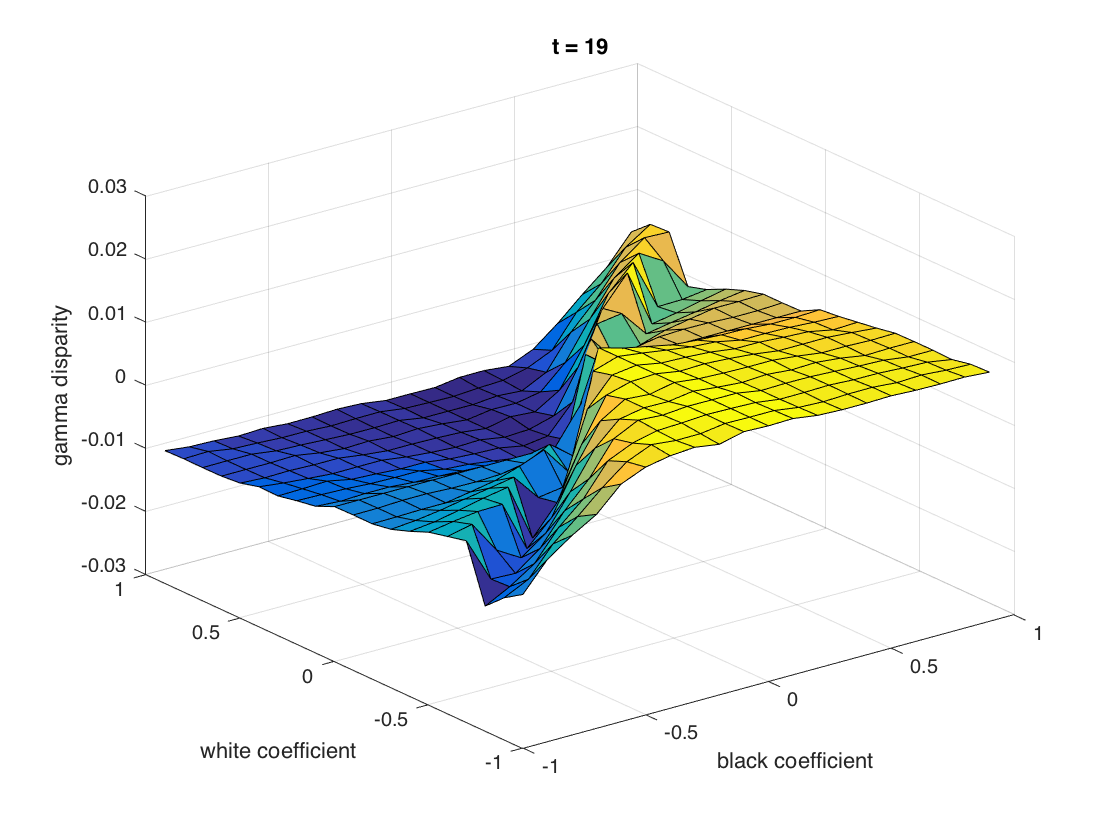
\includegraphics[scale=0.15]{figures/heatfig19.png}}
\subfigure[]{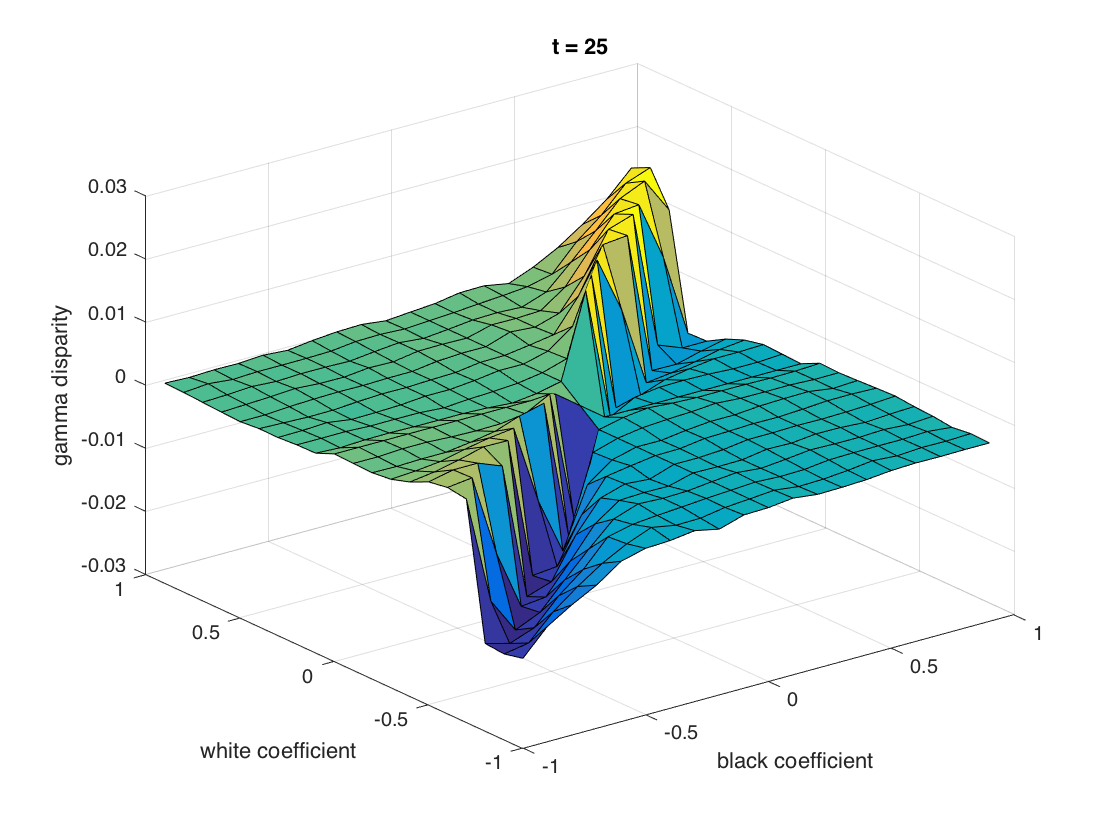
\includegraphics[scale=0.15]{figures/heatfig25.png}}
\subfigure[]{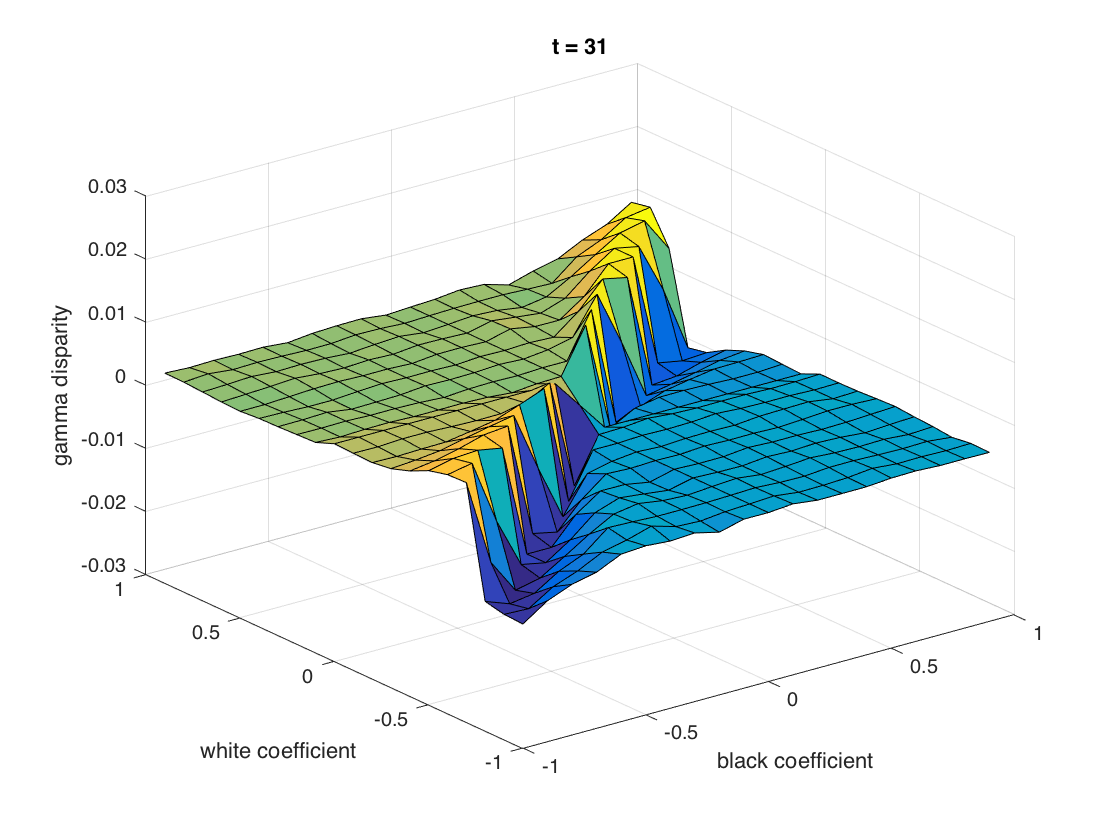
\includegraphics[scale=0.15]{figures/heatfig31.png}}
\subfigure[]{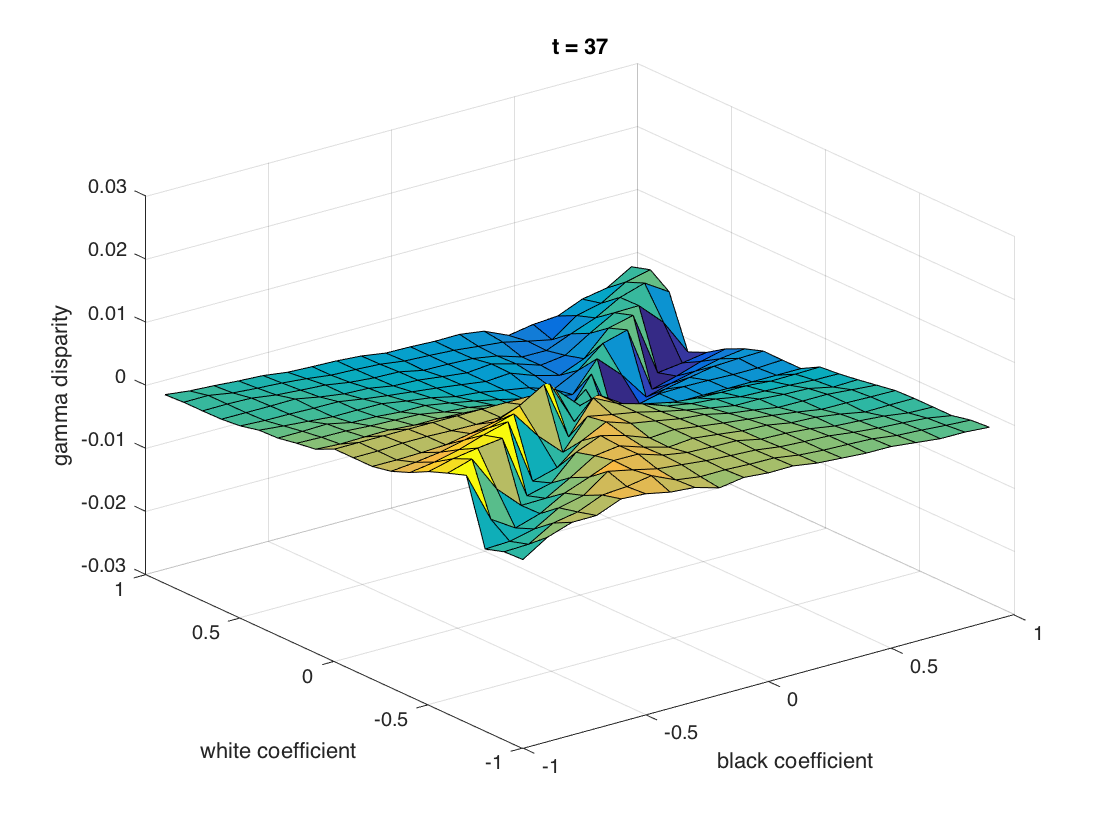
\includegraphics[scale=0.15]{figures/heatfig37.png}}
\hspace{1.75in}
\subfigure[]{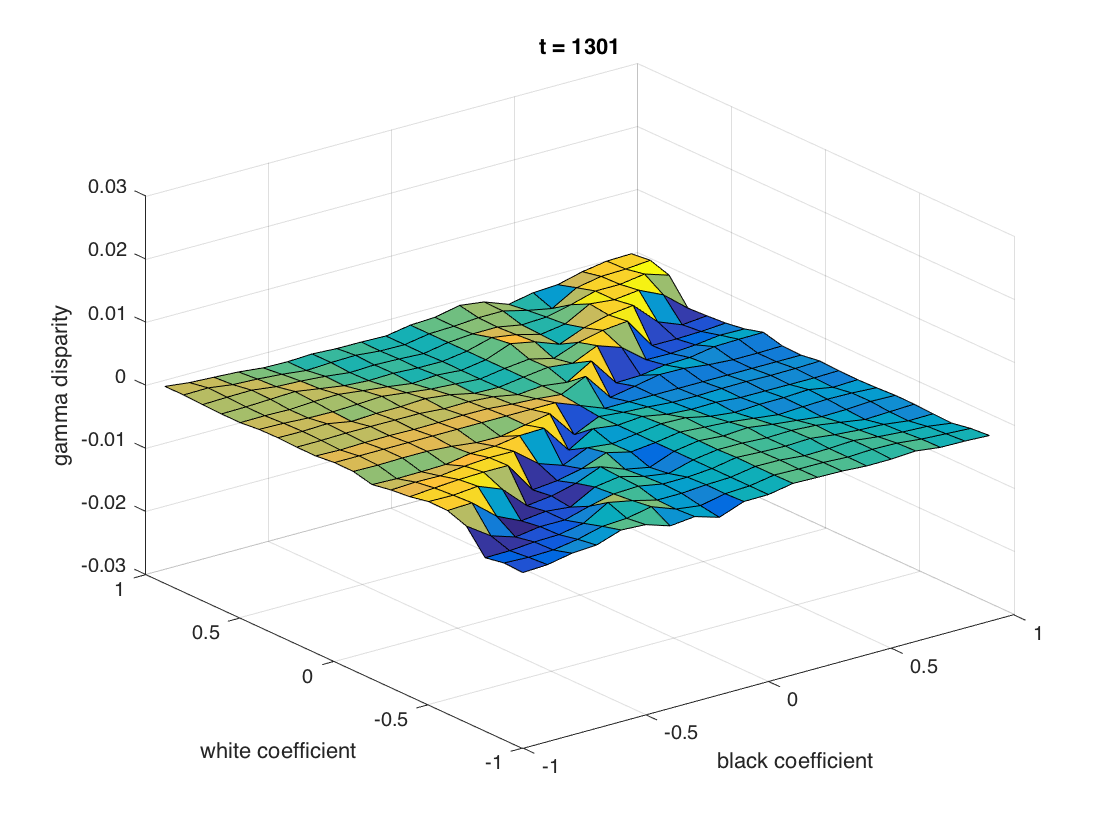
\includegraphics[scale=0.15]{figures/heatfig1301.png}}
\caption{
Evolution of discrimination surface for the $\knrw$ algorithm from $t = 1 \ldots 1301$.
Each point in the plane corresponds to a different subgroup over two protected attributes,
and the corresponding $z$ value is the current false positive discrepancy for the subgroup.
}
\label{fig:heatmap}
\end{figure*}
%\end{center}

Recall that in the various analyses and plots above, we rely on the
Auditor of $\knrw$ to detect unfairness. This Auditor is in turn a heuristic,
relying on an optimization procedure without any theoretical guarantees, which could potentially fail in practice.
This means that while any detected unfairness is a lower bound on the true subgroup unfairness,
it could be the case that the heuristic Auditor is simply failing to detect a larger disparity,
and that the models learned by $\knrw$ look more fair than they really are.

We explore this possibility on the Communities \& Crime dataset by implementing a brute force
Auditor that runs alongside the $\knrw$ algorithm. To make brute force auditing computationally tractable,
we designate only two attributes as protected; \textit{pctwhite} and \textit{pctblack},
the percentage of each community that consists of white and black people respectively.
While the $\knrw$ algorithm uses the same heuristic Auditor it always does,
at each round we also perform a brute force audit as follows.
Subgroups $g_\theta$ are defined by a linear threshold function $\theta$ over the $2$ sensitive attributes, e.g. $(x_1, x_2) \in g_\theta$ iff
$\langle \theta, (x_1, x_2) \rangle \geq 0$. We discretize $\theta \in [-1,1]^2$ in increments of $0.1$, and for the subgroup defined by each $\theta$ in the discretization we compute the $\gamma$-unfairness. Hence at each round we can take the current classifier of the Learner, and plot for each group $g_\theta$ the point $(\theta_1, \theta_2, \gamma)$.

Note that in addition to making brute force auditing tractable, restricting to two dimensions permits direct visualization of discrimination.
In Figure~\ref{fig:heatmap}, we show a sequence of ``discrimination surfaces'' for the $\knrw$ algorithm over the $2$ protected features,
with input $\gamma = 0$. The $x-y$ axes are the coefficients of $\theta$
corresponding to \textit{whitepct} and \textit{blackpct} respectively, and the $z$-axis is the $\gamma$-unfairness of
the corresponding subgroup. This is our first non-heuristic view of $\gamma$-unfairness, and
also shows us the entire surface of $\gamma$-unfairness, rather than just the most violated subgroup.
Note that perfect subgroup fairness would correspond to an entirely flat discrimination surface at $z = 0$.

We observe first that the unconstrained classifier in $t = 1$ (panel (a))
shows a very systematic bias along the lines of our sensitive attributes. In particular groups with \textit{whitepct} $> 0$ and \textit{blackpct} $< 0$, e.g. communities with large numbers of white residents and relatively fewer black residents have a much higher false positive rate for being classified as violent.
Conversely, majority black communities are less likely to be incorrectly labeled as violent.
The mean $\gamma$-unfairness (base rate - community rate) for  \textit{whitepct} $> 0$,  \textit{blackpct} $< 0$
communities is $-0.0242$, whereas the mean for \textit{whitepct} $< 0$,  \textit{blackpct} $ > 0$ groups is
$0.0247$. The maximum $\gamma$-unfairness in $t = 1$ is $0.028$, and $61.25\%$ of the $400$ subgroups have $\gamma$-unfairness $ > 0.02$. Recall that this corresponds to e.g. a $20\%$ disparity of the false positive rate from the base rate, for groups as large as 10\% of the population. 
We are thus far from perfect subgroup fairness.

As the algorithm proceeds, we see this discrimination flip by $t = 7$ (panel (b)),
into a regime with a higher false positive rate for predominantly black communities,
and then revert again by $t = 13$. Over the early iterations these oscillations continue, growing less
drastic as the $\gamma$-unfairness surface starts to flatten out noticeably by $t = 37$ (panel (g)).
In panel (h) we plot $t = 1301$ and see that the surface has almost completely
flattened, with maximum $\gamma$-unfairness below $.0028$.
So over the course of the first $1300$ iterations of $\knrw$ we've reduced the
$\gamma$-unfairness from over $0.02$ in most of the subgroups,
to less than $0.0028$ in \textit{every} subgroup. 
Recall again that this corresponds to false positive rate disparities of at most 2.8\% in subgroups that represent 10\% of the population --- a reduction from false positive rate disparities of 20\% many similarly sized subgroups. This represents an order of magnitude improvement that results from using the classifier learned by $\knrw$. 
%The difference between the unfairness of the unconstrained classifier in panel (a) vs. the classifier learned by $\knrw$ in panel (h)
%could be very meaningful in practice; for example it could be the difference between having many large subgroups
%of weight $10\%$ whose false positive rate is more than $0.2$ from the base rate, vs.
%the statement that \textit{every} subgroup with weight at least $10\%$ has false positive rate within $0.02$ of the base rate,
%an order of magnitude smaller.

\subsection{Understanding the Dynamics}
\label{subsec:traj}

\begin{figure*}[h]
\centering
\subfigure[]{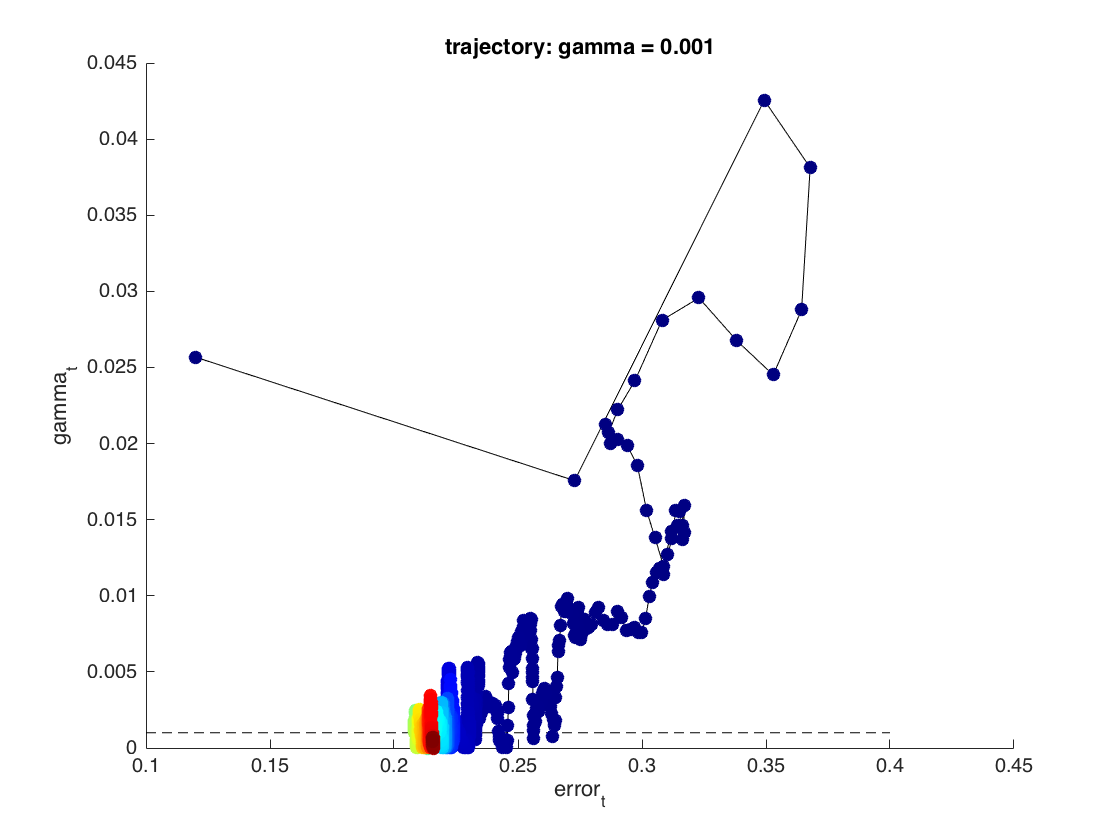
\includegraphics[scale=0.15]{figures/ccgam1.png}}
\subfigure[]{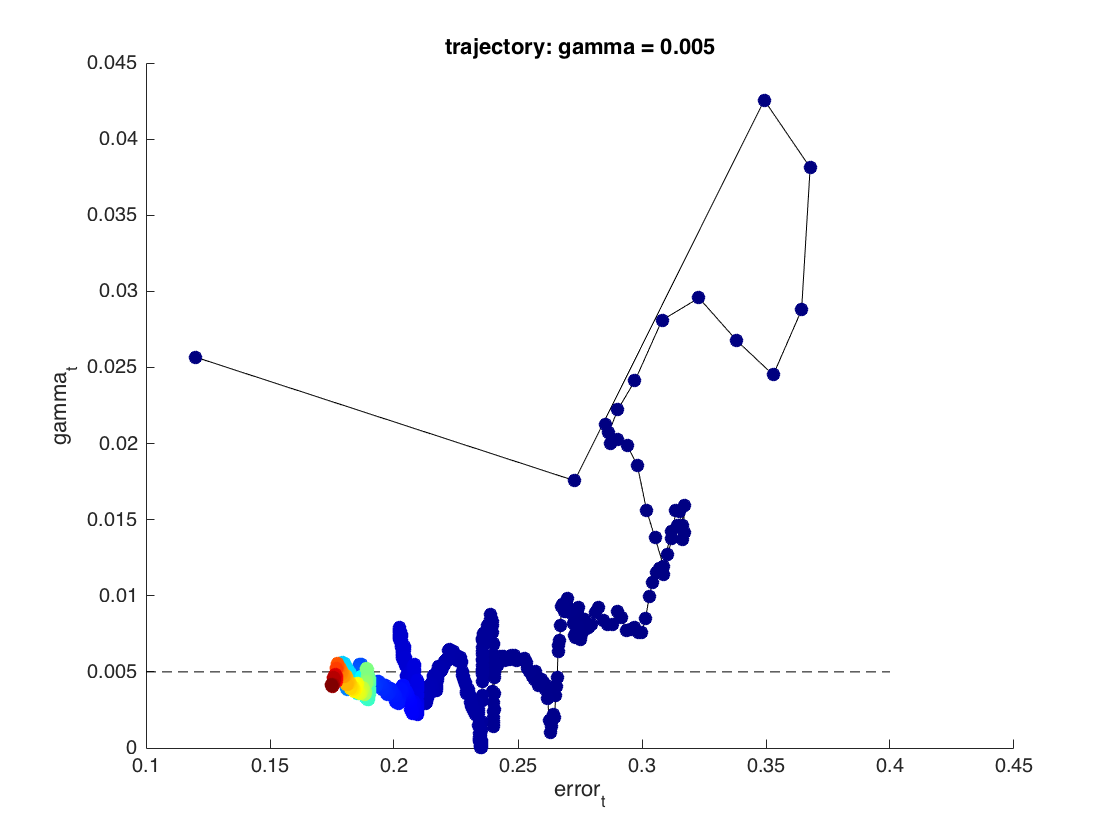
\includegraphics[scale=0.15]{figures/ccgam5.png}}
\subfigure[]{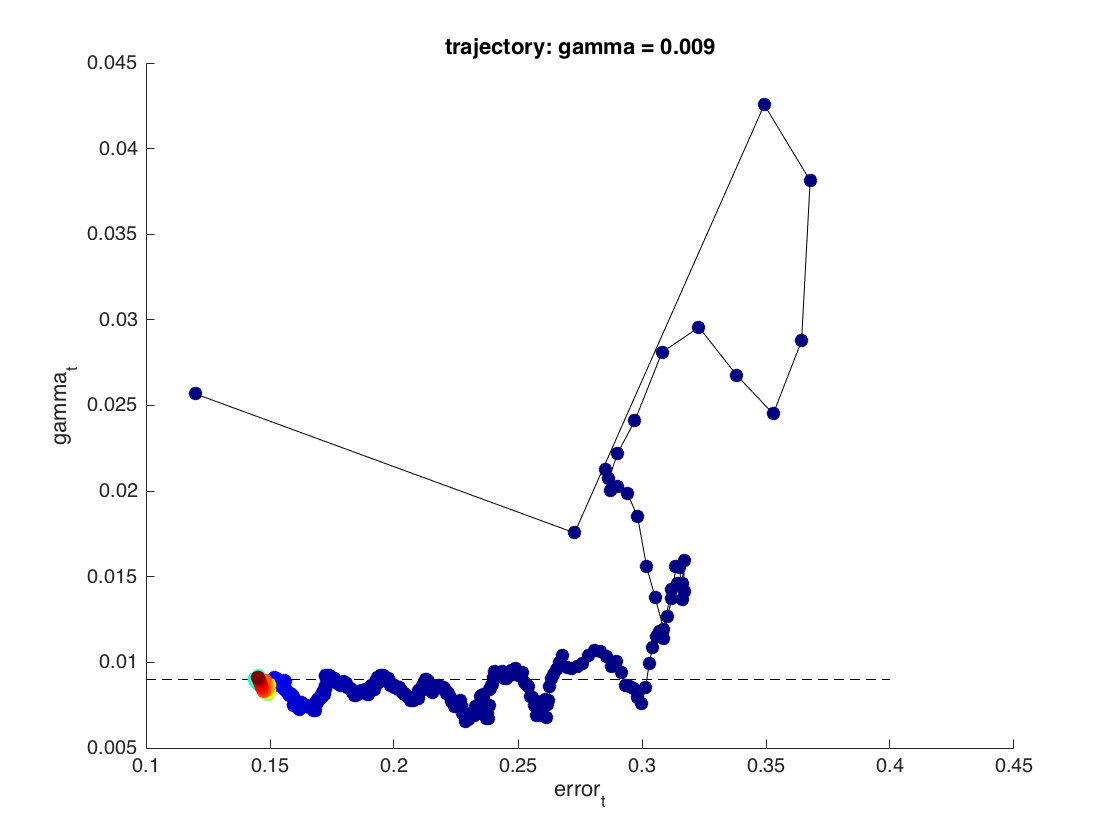
\includegraphics[scale=0.15]{figures/ccgam9.png}}
\subfigure[]{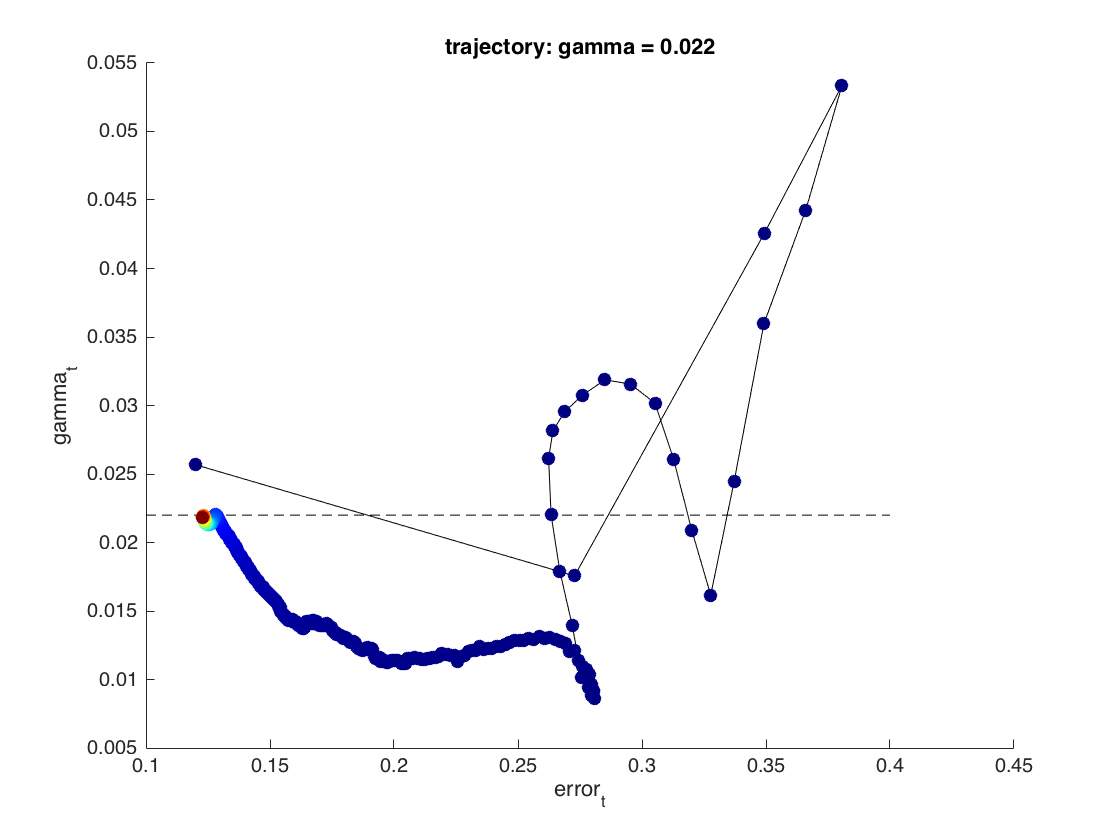
\includegraphics[scale=0.15]{figures/ccgam22.png}}
\caption{
$\langle \epsilon_t, \gamma_t \rangle$ trajectories for
Communities and Crime, for $\gamma \in \{0.001, 0.005, 0.009, 0.022\}.$
}
\label{traj}
\end{figure*}

We conclude by examining the dynamics of the $\knrw$ algorithm on the Communities and Crime dataset in greater detail.
More specifically, since the algorithm is formulated as a game between a Learner who at each iteration $t$ is trying to minimize the
error $\epsilon_t$, and an Auditor who is trying to minimize subgroup unfairness $\gamma_t$, we visualize the trajectories
traced in $\langle \epsilon_t, \gamma_t \rangle$ space as $t$ increases.

The plots in Figure~\ref{traj} correspond to such trajectories for input $\gamma$ values of $0.001, 0.005, 0.009,$ and $0.022$
(panels (a), (b), (c) and (d) respectively), which are
denoted by the dashed lines on the $\gamma_t$ axis of each figure. The $0.001$ and $0.005,0.009$ values correspond to small
and intermediate $\gamma$ regimes, whereas $0.022$ is close to (but slightly below)
the subgroup unfairness of the unconstrained classifier. The trajectories are color coded from colder
to warmer colors according to their iteration number to give a sense of speed of convergence.

The first plot in all four trajectories corresponds to the
$\langle \epsilon_0, \gamma_0 \rangle$
of the unconstrained classifier. Furthermore, as long as the current $\gamma_t$ values remain above the
horizontal dashed line representing the input $\gamma$, the trajectories remain identical, as the same subgroups are
being presented to the learner in each trajectory. But when $\gamma_t$ falls below a given input $\gamma$, that
trajectory will follow its own path going forward.

We first observe that the dynamics exhibit a fair amount of complexity and subtlety. They all begin with low error and
large unfairness, and quickly follow a brief but large increase in $\epsilon_t$ as fairness starts to be enforced. There
are steps in which both $\epsilon_t$ and $\gamma_t$ increase, and a large early loop in trajectory space is observed.
But the first three trajectories (panels (a), (b) and (c), corresponding to the three smaller values of $\gamma$) quickly settle near the
input $\gamma$ line, at which point begins a long, oscillatory ``border war'' around this line, as the Learner tries to minimize
error, but is pushed back below the line by the Auditor anytime $\gamma$-fairness is violated. The idealized theory predicts
that each trajectory should end at the input $\gamma$ line (subgroup fairness constraint saturated), and with larger
input $\gamma$ (weaker fairness constraint) resulting in lower error. The empirical trajectories indeed conform nicely
to the theory, with the final (red) points near the dashed lines, and further left for larger $\gamma$.

Panel (d), corresponding to a much larger input $\gamma$, diverges much earlier from the other three (on its second step),
and early on sees unfairness driven far below the specified value. The dynamics then see a slow, gradual decrease of
error and increase of unfairness back to the input value, with the trajectory ending up near where it began, but just
slightly more fair, as specified by $\gamma$.


%%% Local Variables:
%%% mode: latex
%%% TeX-master: "main.tex"
%%% End:
